%%%
%
% $Autor: Wings $
% $Datum: 2021-05-14 $
% $Pfad: GitLab/MLEdgeComputer $
% $Dateiname: GearDrive
% $Version: 4620 $
%
% !TeX spellcheck = de_DE/GB
% !TeX program = pdflatex
% !BIB program = biber/bibtex
% !TeX encoding = utf8
%
%%%



\chapter{Getriebemotor mit Rad}

Für den Antrieb werden zwei Getriebemotoren mit Rädern von JOY-IT verwendet. Es handelt sich um einen Getriebemotor mit großem Spannungsbereich und beidseitiger Welle. Der Motor ist in Abbildung \ref{fig:motor} zu sehen. Die technischen Daten sind in den Tabellen \ref{tab:general_info_gear_motor} und \ref{tab:gear_motor_specs} dargestellt. \cite{Simac:2018}

\begin{figure}
    \centering
    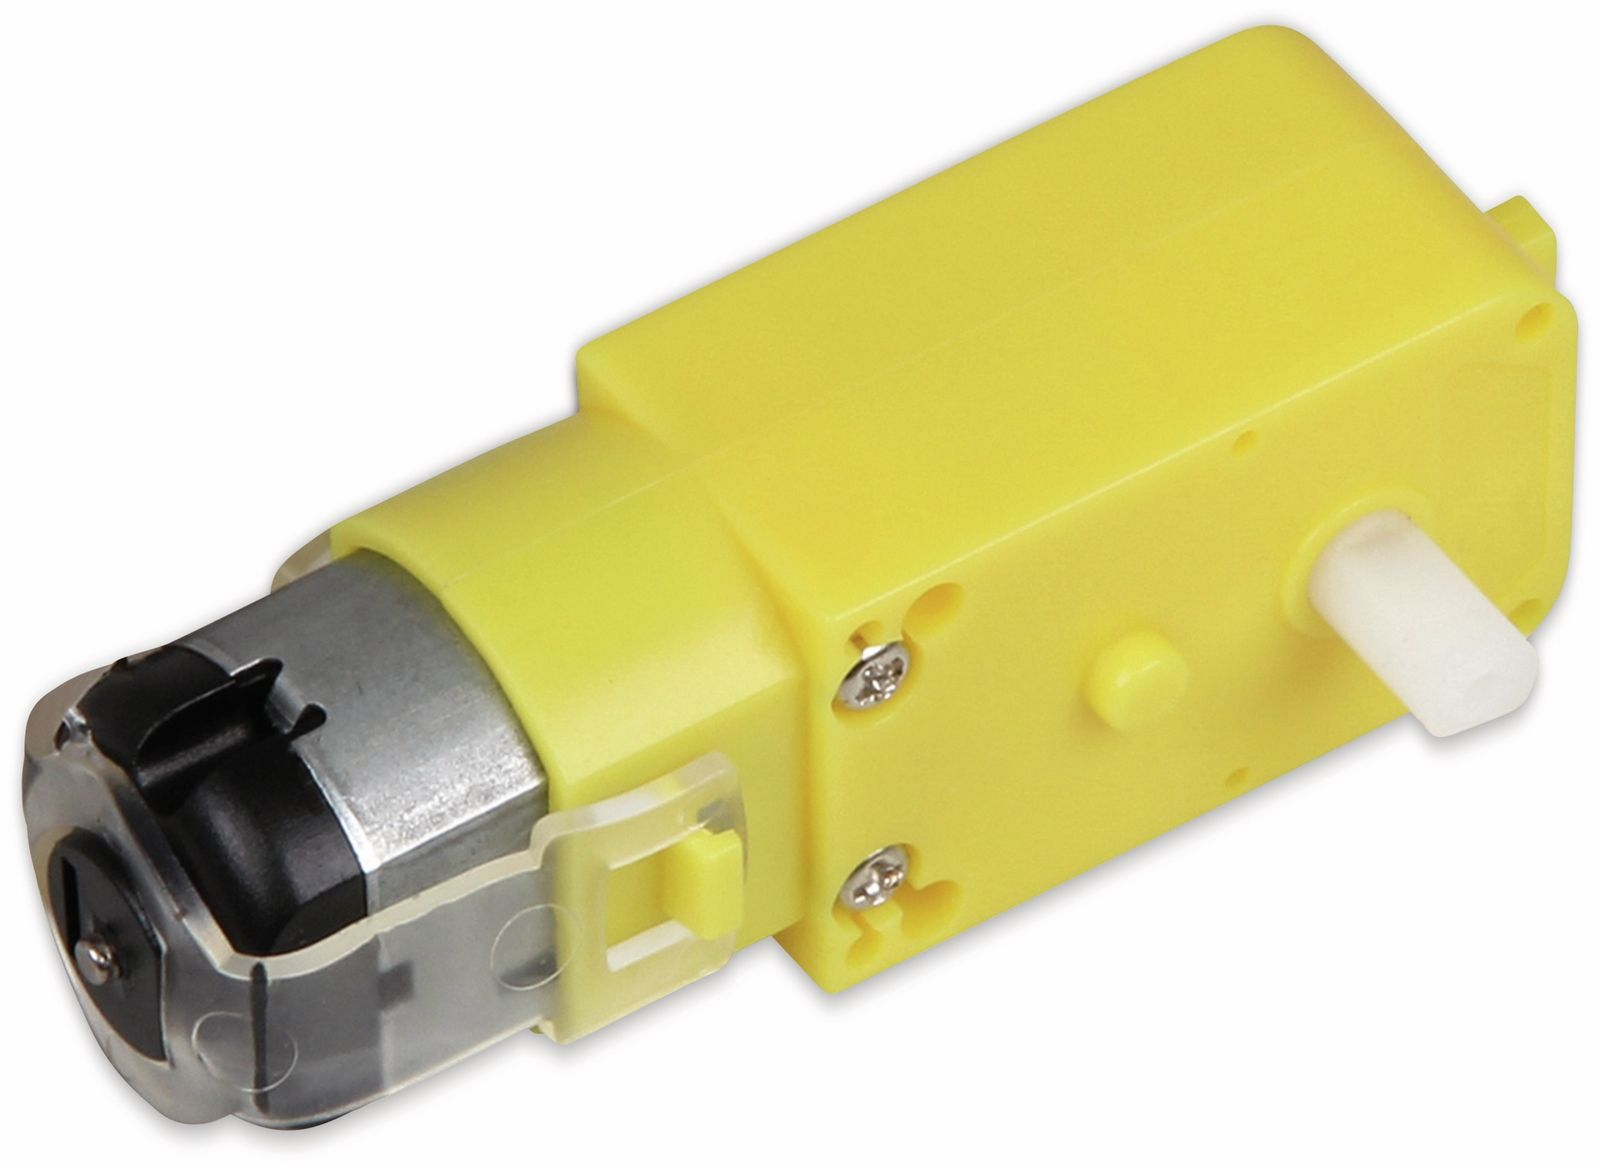
\includegraphics [width=70mm] {GearDrive/GearDrive}
    \caption{Getriebemotor}
    \label{fig:motor}
\end{figure}


\begin{table}
    \centering
    \begin{tabular}{|l|l|}
        \hline
        \textbf{Eigenschaft}           & \textbf{Wert}                          \\ \hline
        Welle                          & 3,6mm beidseitig mit Loch 1,9mm        \\ 
        Spannungsversorgung            & 3 - 9V DC (empfohlen: 4,5V)            \\ 
        \begin{tabular}[c]{@{}l@{}}Abmessungen (Rad)\\ Durchmesser\\ Breite\end{tabular} & \begin{tabular}[c]{@{}l@{}}65mm\\ 27mm\end{tabular} \\ 
        Abmessungen (Motor)            & 37,6 x 64,2 x 22,5mm                   \\ \hline
    \end{tabular}
    \caption{Allgemeine Informationen des Getriebemotors mit Rad}
    \label{tab:general_info_gear_motor}
\end{table}
\begin{table}
    \centering
    \begin{tabular}{|l|c|c|c|c|}
        \hline
        \textbf{Spannung DC (V)}&4,5  & 6 &7,2&9  \\ \hline
        \textbf{Stromstärke im Leerlauf (mA)}&190&160&180&200       \\ \hline
        \textbf{Drehzahl pro Min. im Leerlauf (± 10\%)}& 90&190&230&300  \\ \hline 
        \textbf{Drehmoment (gf/cm)} &800 &800  &1000&1200 \\ \hline
    \end{tabular}
    \caption{Technische Daten des Getriebemotors mit Rad}
    \label{tab:gear_motor_specs}
\end{table}

\section{Funktion Motoren}

Nachdem der Roboter nach Anleitung aufgebaut ist, kann durch Laden des folgenden Codes \ref{motortest} auf den Arduino getestet werden, ob die Motoren richtig angeschlossen sind und funktionieren. Es ist wichtig, dass beide Motoren in die selbe Richtung drehen, ansonsten ist die Verkabelung zu überprüfen.



\begin{lstlisting}[caption=Arduino Motor Test, label=motortest, language=C++]
    // Motorsteuerungs-Pins
    const int in1 = 6;
    const int in2 = 9;
    const int in3 = 10;	const int in4 = 11;
    
    // Funktion zum Vorwaertsfahren der Motoren
    void forward(int geschw) {
        analogWrite(in1, geschw);
        analogWrite(in2, 0);
        analogWrite(in3, geschw);
        analogWrite(in4, 0);
        
        Serial.print("Motoren vorwaerts: Geschwindigkeit = ");
        Serial.println(geschw);
    }
    
    // Funktion zum Rueckwaertsfahren der Motoren
    void backward(int geschw) {
        analogWrite(in1, 0);
        analogWrite(in2, geschw);
        analogWrite(in3, 0);
        analogWrite(in4, geschw);
        
        Serial.print("Motoren rueckwaerts: Geschwindigkeit = ");
        Serial.println(geschw);
    }
    
    // Funktion zum Stoppen der Motoren
    void stopMotors() {
        analogWrite(in1, 0);
        analogWrite(in2, 0);
        analogWrite(in3, 0);
        analogWrite(in4, 0);
        
        Serial.println("Motoren gestoppt");
    }
    
    void setup() {
        // Initialisierung der seriellen Kommunikation 
        // fuer Debugging
        Serial.begin(9600);
        
        // Konfigurieren der Motorsteuerungspins als Ausgaenge
        pinMode(in1, OUTPUT);
        pinMode(in2, OUTPUT);
        pinMode(in3, OUTPUT);
        pinMode(in4, OUTPUT);
    }
    
    void loop() {
        // Motoren fuer 5 Sekunden vorwaerts fahren
        Serial.println("Motoren fahren vorwaerts");
        forward(255); // Volle Geschwindigkeit
        delay(5000);  // 5 Sekunden warten
        
        // Motoren fuer 5 Sekunden rueckwaerts fahren
        Serial.println("Motoren fahren rueckwaerts");
        backward(255); // Volle Geschwindigkeit
        delay(5000);   // 5 Sekunden warten
        
        // Motoren fuer 5 Sekunden anhalten
        Serial.println("Motoren anhalten");
        stopMotors();
        delay(5000);   // 5 Sekunden warten
    }
    
\end{lstlisting}
